\chapter{Requirement definitions}

\section*{Introduction}

After imbibing the general context of the project, we are going to focus in
the is chapter on providing a full description of out project, that we will be
calling Benchmarks Dashboard. To do so, we will start by analyzing the
requirements and extracting the  functional and non-functional specifications.
Then we will define the Product backlog of the project to achieve. Finally we
will present the general use cases of the project.

\pagebreak

\section{Requirements analysis}

\subsection{Design session}
After  the beginning of the internship, we had a on-month training where we were
trained about the different technologies that Predictix is using, such as
LogiQL, Nix and LB. Also, as interns, we had the opportunity, first, to get
familiar with the company's working environment, second, understand better the
project's goal and its added value to its users, and third, were able to collect
the functional and non functional requirements of the project.


\subsection{Functional requirements}
The  purpose of this project is to automate the benchmarking process of the
applications developed in Predictix. For that there are two main requirements
that need to be addressed.

\subsubsection{Automating "benchmark runs"}
The application should give the ability to the clients, the developers, to run
benchmark with the click of a button. The application must run all the repeated
process without user's interactions. For that 3 operations must be automated:

$\bullet$ \textbf{Deploy the application}: The applications developed in house
are SaaS applications, thus they must be deployed to the cloud. The user choose
what the application that want to run benchmark for. Then we need to automatically
provision a server in the cloud, install the application on that server along
with all dependencies that are needed to run the benchmark.

$\bullet$ \textbf{Load test data}: To have a real and concise measure of the
performance of the application, a data sample should be loaded into the
database. This sample should be the same across all benchmarks runs so it can
make sense to compare them. The data should be loaded as soon as the application
is installed.

$\bullet$ \textbf{Run The benchmark}: After loading test data we will run a
series of service test and measure the time each service took to complete the
request. Each service test will be run 3 times to unveil any issues with
database warmup.

Finally after the benchmarks completed the result of the test should be stored
for the developer to check and the instance should not be provisioned. The figure
\hyperref[fig:bpmn-new-benchmark]{\ref{fig:bpmn-new-benchmark}} shows the BPMN diagram
of "New Benchmark" process.

\begin{figure}[h]
  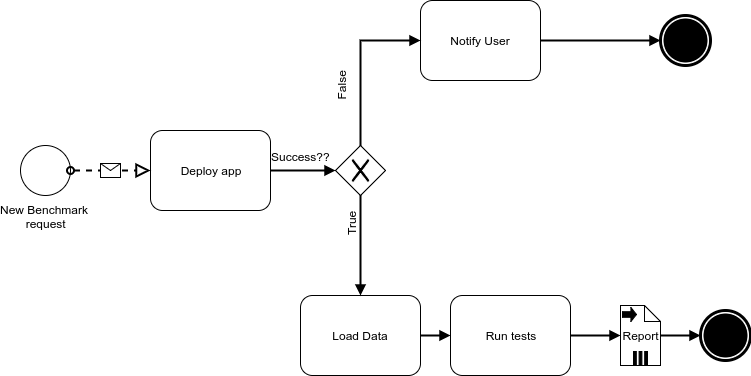
\includegraphics[width=14cm]{bpmn-new-benchmark}
\caption{BPMN diagram: New benchmark}
\label{fig:bpmn-new-benchmark}
\end{figure}

\subsubsection{Visualize the previous benchmarks}
The developer should be able to see and investigate the result of the
benchmarks. He must be also be able to:

$\bullet$ \textbf{Compare benchmarks}: In this case the user can see difference
in the overall performance of the application, between two different dates.

$\bullet$ \textbf{Test history}: The user can see the test history. Thus the
state of the test between all benchmarks, or specify two bencharmks.

$\bullet$ \textbf{Benchmark status}: The user can see the status of the
benchmark. Whether they competed successfully or not or they still running. Also
they can see who started the benchmark run, and when he started it.

\section{Product Backlog}
From the previous requirements and some other related to user management we can
extract the product backlog described in table \hyperref[product-backlog]{\ref{product-backlog}}

\begin{table}[!hp]
\caption{Product Backlog}
\label{product-backlog}
\centering
  \begin{tabular}{ | p{2cm}  | p{7cm}  | p{2cm} | p{2cm}| }
    \hline

    ID & User Story                                                                                                        & Priority        & Estimation\\ \hline

    1 & As a user, I want to login using my username and password and start using the application right away.              & 2              & 14        \\ \hline
    2 & As a user, I want to visualize account’s applications and select one to run new benchmark                          & 1              & 20        \\ \hline
    3 & As a user, I want to visualize the list of accounts.                                                               & 4              & 3        \\ \hline
    4 & As a user, I want to visualize the status of account’s benchmarks.                                                 & 7              & 8       \\ \hline
    5 & As a user, I want to be able to choose an account and visualize it’s history                                       & 5              & 14        \\ \hline
    6 & As a user, I want to be able to choose a benchmark and visualize the tests duration.                              & 6              & 6        \\ \hline
    7 & As a user, I want to be able to choose a test in an account and visualize the history over all benchmarks.         & 8              & 8       \\ \hline
    8 & As an account administrator, I want to be able to grant ‘Run benchmark’ right to users also be able to revoke it. & 9              & 4        \\ \hline
    9 & As an administrator, I want to be able to manage all accounts.                                                    & 3              & 3       \\ \hline

    \hline
  \end{tabular}
\end{table}

Once the Product backlog was established and validated by the Product Owner, the
scrum team has broken down the Product Backlog into four sprints of a duration
of 20 days each. The sprint duration was suggested by the Scrum Master as sprint
ceremonies were planned every 20 days at the end of each sprint.

The table \hyperref[sprints]{\ref{sprints}} defines the user stories that will
be achieved during each sprint.

\begin{table}[]
\centering
\label{sprints}
\begin{tabular}{|p{2cm}|p{7cm}|p{2cm}|}
                           \hline
                              &  User stories & Estimation \\ \hline
Sprint 1                      &  As a user, I want to visualize account’s applications and select one to run new benchmark &  20\\ \hline

{\multirow{2}{*}{}} Sprint 2  &  As a user, I want to login using my username and password and start using the application right away.  &  14\\ \cline{2-3}
{}                            &  As an administrator, I want to be able to manage all accounts. &  3\\ \cline{2-3}
{}                            &  As a user, I want to visualize the list of accounts. &  3\\ \hline

{\multirow{3}{*}{}} Sprint 3  &  As a user, I want to be able to choose a test in an account and visualize the history over all benchmarks.& 14 \\ \cline{2-3}
{}                            &  As an account administrator, I want to be able to grant ‘Run benchmark’  right to users also be able to revoke it.&  6\\ \hline
{\multirow{3}{*}{}} Sprint 4  &  As a user, I want to visualize the status of account’s benchmarks. & 8 \\ \cline{2-3}
{}                            &   As a user, I want to be able to choose a test in an account and visualize the history over all benchmarks. & 8  \\ \cline{2-3}
{}                            &  As an account administrator, I want to be able to grant ‘Run benchmark’  right to users also be able to revoke it&  4\\ \hline

\end{tabular}
\caption{User Stories through each sprint}
\end{table}
\section{Requirement specifications}
\subsection{Actors identification}
The intended users of the Benchmarks Dashboard are Predictix employees, The
AppDev team (Application development team). They must be able to, easily
Interact with the system, run new benchmarks and check the status and result as
soon as possible.

\begin{itemize}
  \item{\textbf{AppDev team}}: The AppDev members are the developer that implement new
    feature in the application, write the necessary steps to build the
    application and monitor the performance of the application after every new
    feature.
  \item{\textbf{Account admin}}: The account admin will be responsible for managing
    account users. Grant run benchmark rights and revoke them.
  \item{\textbf{Administrator}}: the administrator is a person who should be chosen,
    carefully. in fact, s/he will be creating, editing and deleting users,
    accounts. The administrator should also be able to assign accounts to users.
\end{itemize}

\subsection{Use case diagram}
The figure \hyperref[fig:use-case]{\ref{fig:use-case}} introduces the general use cases which present the
functionalities of the application.

\begin{figure}[h]
  \center
  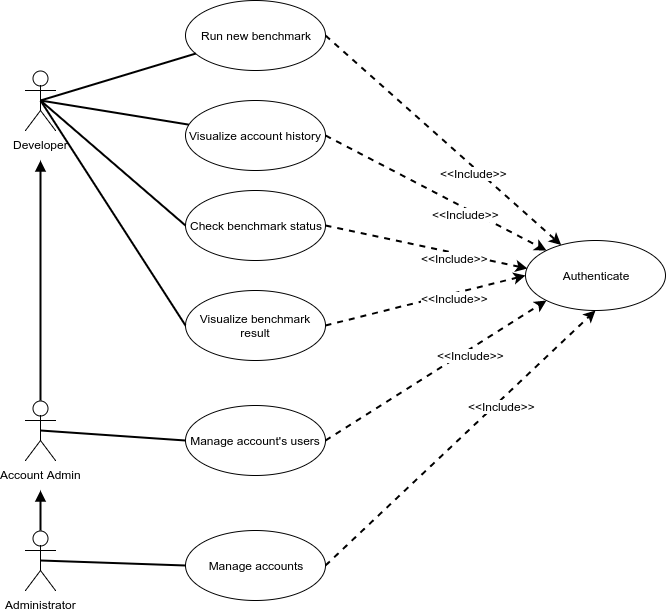
\includegraphics[width=14cm]{use-case}
  \caption{General use case diagram}
\label{fig:use-case}
\end{figure}


\section*{Conclusion}
